\documentclass{beamer}
\usepackage{amsmath}
\usepackage{graphicx}
\usepackage{listings}
\usepackage{amsmath}
\usepackage{amssymb}
\usepackage{booktabs}
\usepackage{tikz}

\title{Analisi di Sensibilità e Ottimizzazione dei Parametri}
\author{Lorenzo Principi}
\date{\today}

\begin{document}

\frame{\titlepage}

\begin{frame}
    \frametitle{Introduzione}

    \begin{equation}
        P(rate_{fp} + rate_{tp} > th)
    \end{equation}

\end{frame}



\begin{frame}
    \frametitle{Introduzione}

    \begin{align}
        rate_{fp} &= \mathcal{N}_{fp}(\mu_{fp}, \sigma_{fp}) \\
        rate_{tp} &= \mathcal{N}_{tp}(\mu_{tp}, \sigma_{tp})
    \end{align}
    
\end{frame}



\begin{frame}
    \frametitle{Introduzione}
    \begin{itemize}
        \item FPA, False Positive Alert:
    \end{itemize}

    \begin{equation}
        P(rate_{fp} + rate_{tp} \ge th) \cap P(rate_{tp} = 0)
    \end{equation}
\end{frame}



\begin{frame}
    \frametitle{Introduzione}
    \begin{itemize}
        \item TPA, True Positive Alert:
    \end{itemize}

    \begin{equation}
        P(rate_{fp} + rate_{tp} > th) \cap P(rate_{tp} > 0)
    \end{equation}
\end{frame}






\begin{frame}
    \frametitle{Simulazione}
    Si generano randomicamente:
    \begin{itemize}
        \item $n$ false positives (\textit{fps}).
        \item $m$ true positives (\textit{tps}), $m < n$.
    \end{itemize}
    adottando una distribuzione normale $\mathcal{N}(\mu,\sigma)$.
\end{frame}


\begin{frame}
    \frametitle{Simulazione /2}

    Si utilizzano i seguenti parametri:
    \begin{itemize}
        \item $\mu_{fp}$ viene scelta arbitrariamente e mantenuta fissa.
        \item $\sigma_{fp}$ viene ottenuta dal rapporto $\sigma_{fp}/\mu_{fp}$, il
        quale varia in un insieme di valori come, ad esempio, $\{0.1,
        0.5, 1.0, 2.0 \}$.
        \item $\mu_{tp}$ viene ottenuta dal rapporto $\mu_{tp}/\mu_{fp}$, il quale varia in un insieme di valori
        come, ad esempio, $\{0.5, 1.0, 3.0\}$.
        \item $\sigma_{tp}$ si ottiene allo stesso modo di $\sigma_{fp}$.
    \end{itemize}

    \begin{center}
        \begin{tabular}{l||l|l}
            parametro & calcolo & set \\\midrule
            $\mu_{fp}$ & arbitrario e fisso & $\mu_{fp} \in {100}$ \\
            $\mu_{tp}$ & $=\mu_{fp} * \mu_{r}$ & $\mu_{r}=\mu_{tp}/\mu_{fp} \in \{0.5, 1, 3 \}$ \\
            $\sigma_{fp}$ & $=\mu_{fp} * r_{fp}$ & $r_{fp}=\sigma_{fp}/\mu_{fp} \in \{0.1,
            0.5, 1, 2 \}$ \\
            $\sigma_{tp}$ & $=\mu_{tp} * r_{tp}$ & $r_{tp}=\sigma_{tp}/\mu_{tp} \in \{0.1,
            0.5, 1, 2 \}$ \\
        \end{tabular}
    \end{center}
\end{frame}

\begin{frame}
    \frametitle{Simulazione /3}

    \begin{itemize}
        \item \textbf{Calcolo della ROC curve} per ogni set di parametri: la ROC curve analizza tutte le soglie disponibili $th$ e mostra quali
        valori di FPR e TPR si ottengono per ciascuna di esse.
        \item \textbf{Limitazione FPR}: siccome nella NIDS il numero di falsi positivi deve essere minimo, la
        ROC curve che varia tra $0.0$ e $1.0$ è qui limitata a $0.0$ e $0.25$.
    \end{itemize}
\end{frame}

\begin{frame}[plain]
    \begin{tikzpicture}[remember picture,overlay]
        \node[at=(current page.center)] {
            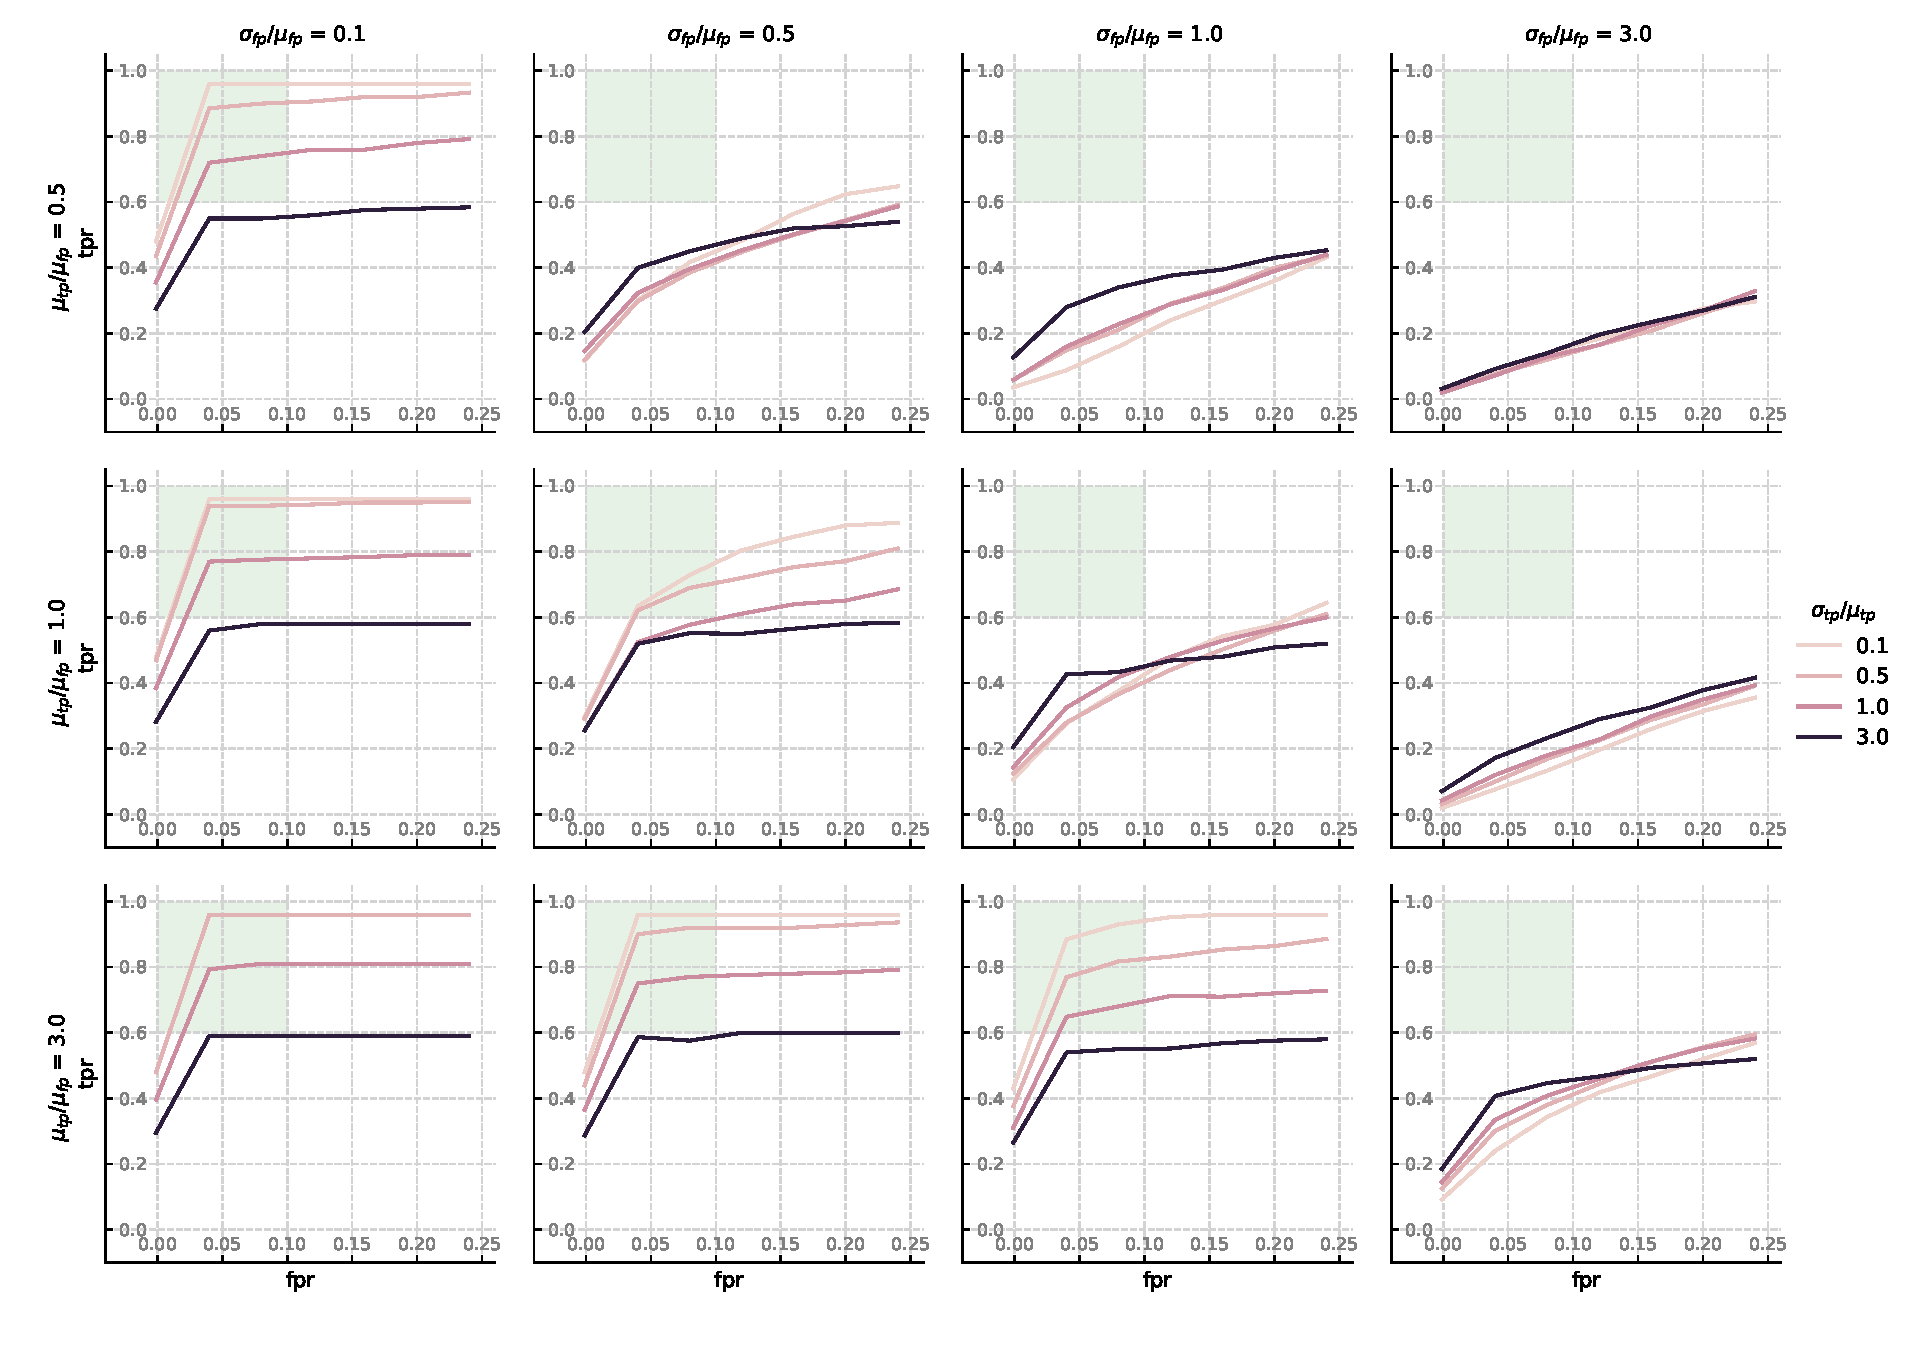
\includegraphics[width=\paperwidth]{simulation.pdf}
        };
    \end{tikzpicture}
\end{frame}



\begin{frame}
    \frametitle{Simulazione con \textit{tps} veri}
    \begin{itemize}
        \item \textbf{Capture reali}: invece di generare i \textit{tps}, utilizziamo le capture di Stratosphere.
        \item \textbf{Suddivisione in slot}: si suddivide la timeline di ogni capture in slot (finestre
        temporali adiacenti di lunghezza fissa).
        \item Ogni slot contiene:
        \begin{itemize}
            \item Il numero di predicted positive ($pp$), ovvero numero di domini
            per cui la rete LSTM ha calcolato una probabilità $> 0.5$ di essere
            DGA-generated.
        \end{itemize}
    \end{itemize}
\end{frame}



\begin{frame}
    \frametitle{Simulazione con \textit{tps} veri /2}
    \begin{itemize}
        \item \textbf{Si considerano $w$-slots} di \textit{tps}.
        \item \textbf{Si generano $w$-slots di fps}, randomicamente adottando una distribuzione normale.
        \item \textbf{Overlapping di fps e tps}: si calcola la \textbf{curva ROC}.
        \item \textbf{Rolling con step di uno slot}: si esegue questo \textit{overlap} per tutta la timeline della capture
        malevola, scorrendo di uno slot per volta.
    \end{itemize}
\end{frame}



\begin{frame}
    \frametitle{Simulazione con \textit{tps} veri /3}
    In questo caso i parametri precedenti saranno:
    \begin{itemize}
        \item $\mu_{tp_{i}}$ e $\sigma_{tp_{i}}$: calcolati dai dati reali della
        $i$-esima finestra.
        \item $\mu_{fp}=\mu_r \cdot \mu_{tp_{i}}$: quindi $\mu_{fp}$ viene
        ottenuto da $\mu_{tp_{i}}$.
        \item $\sigma_{fp}$ viene calcolato allo stesso modo di prima.
    \end{itemize}
    I parametri che possiamo variare sono quindi:
    \begin{itemize}
        \item $\mu_r$, per ottenere $\mu_{fp}$ da $\mu_{tp}$.
        \item $r_{fp}$, per ottenere $\sigma_{fp}$ da $\mu_{fp}$.
    \end{itemize}
\end{frame}



\begin{frame}
    \frametitle{Simulazione con \textit{tps} veri /4}
    Abbiamo scelto 4 capture per i seguenti malware:
    \begin{itemize}
        \item caphaw, simda, unknown, zbot.
    \end{itemize}
    , con i seguenti parametri:
    \begin{itemize}
        \item $\mu_{r} = \mu_{tp}/\mu_{fp} \in \{ 0.5, 1.0, 1.5\}$.
        \item $r_{fp} = \sigma_{fp}/\mu_{fp} \in \{ 0.1, 0.5, 1, 2, 4 \}$.
    \end{itemize}
\end{frame}




\begin{frame}[plain]
    \begin{tikzpicture}[remember picture,overlay]
        \node[at=(current page.center)] {
            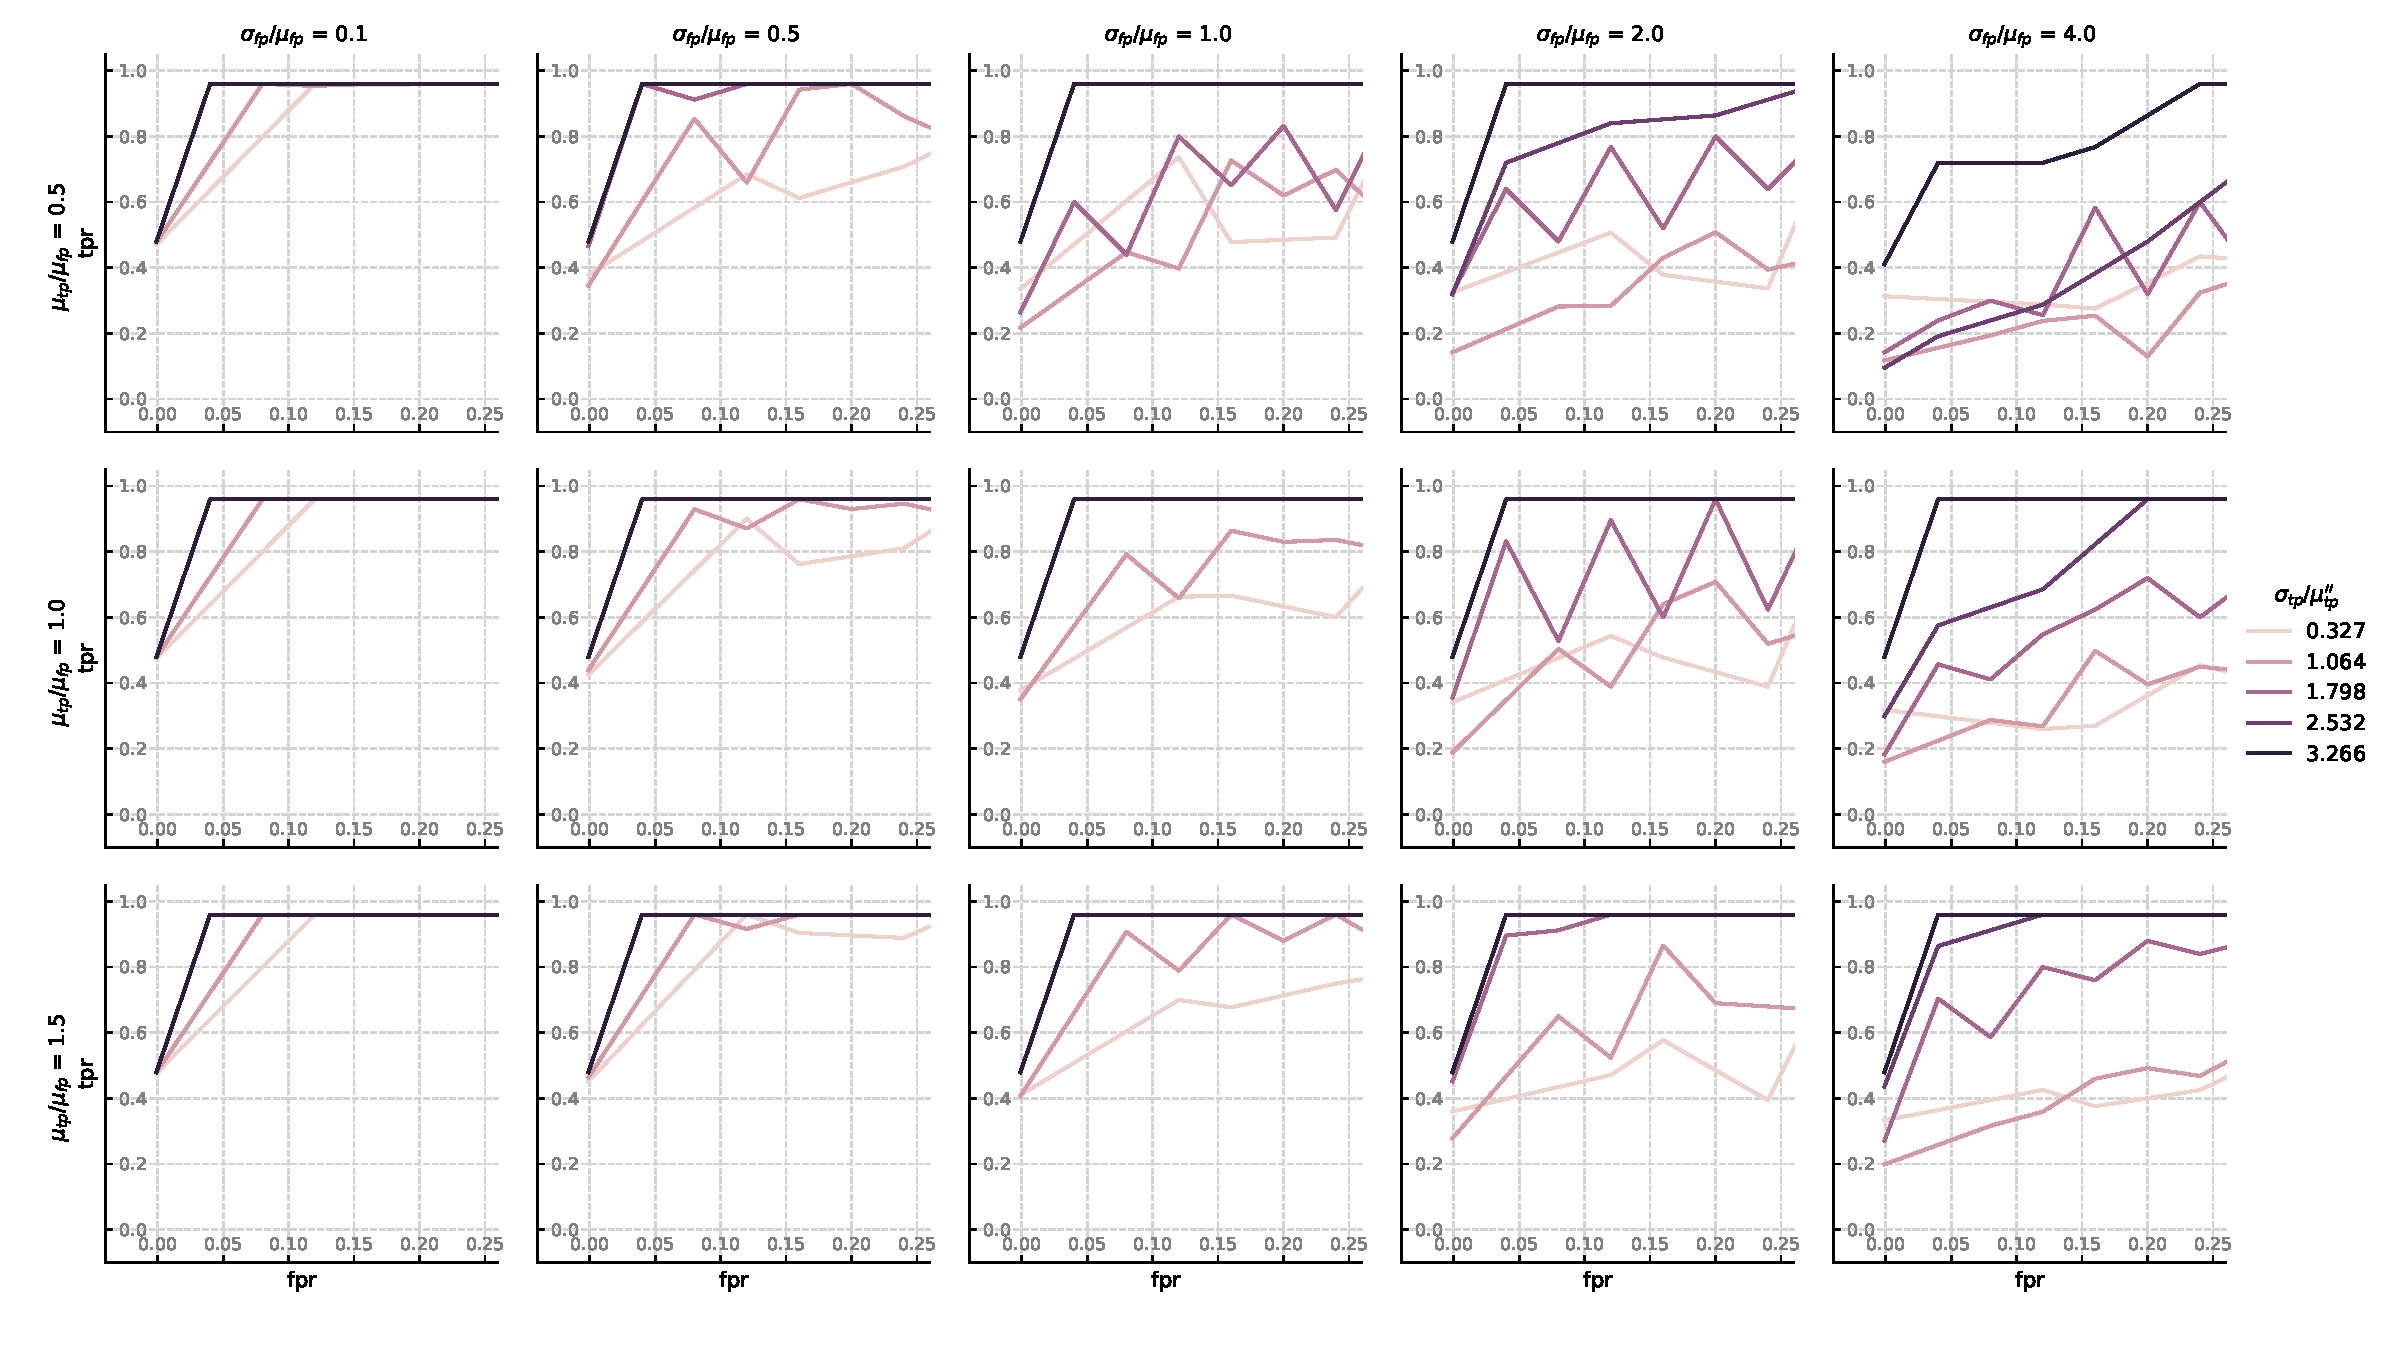
\includegraphics[width=\paperwidth]{caphaw.pdf}
        };
    \end{tikzpicture}
\end{frame}



\begin{frame}[plain]
    \begin{tikzpicture}[remember picture,overlay]
        \node[at=(current page.center)] {
            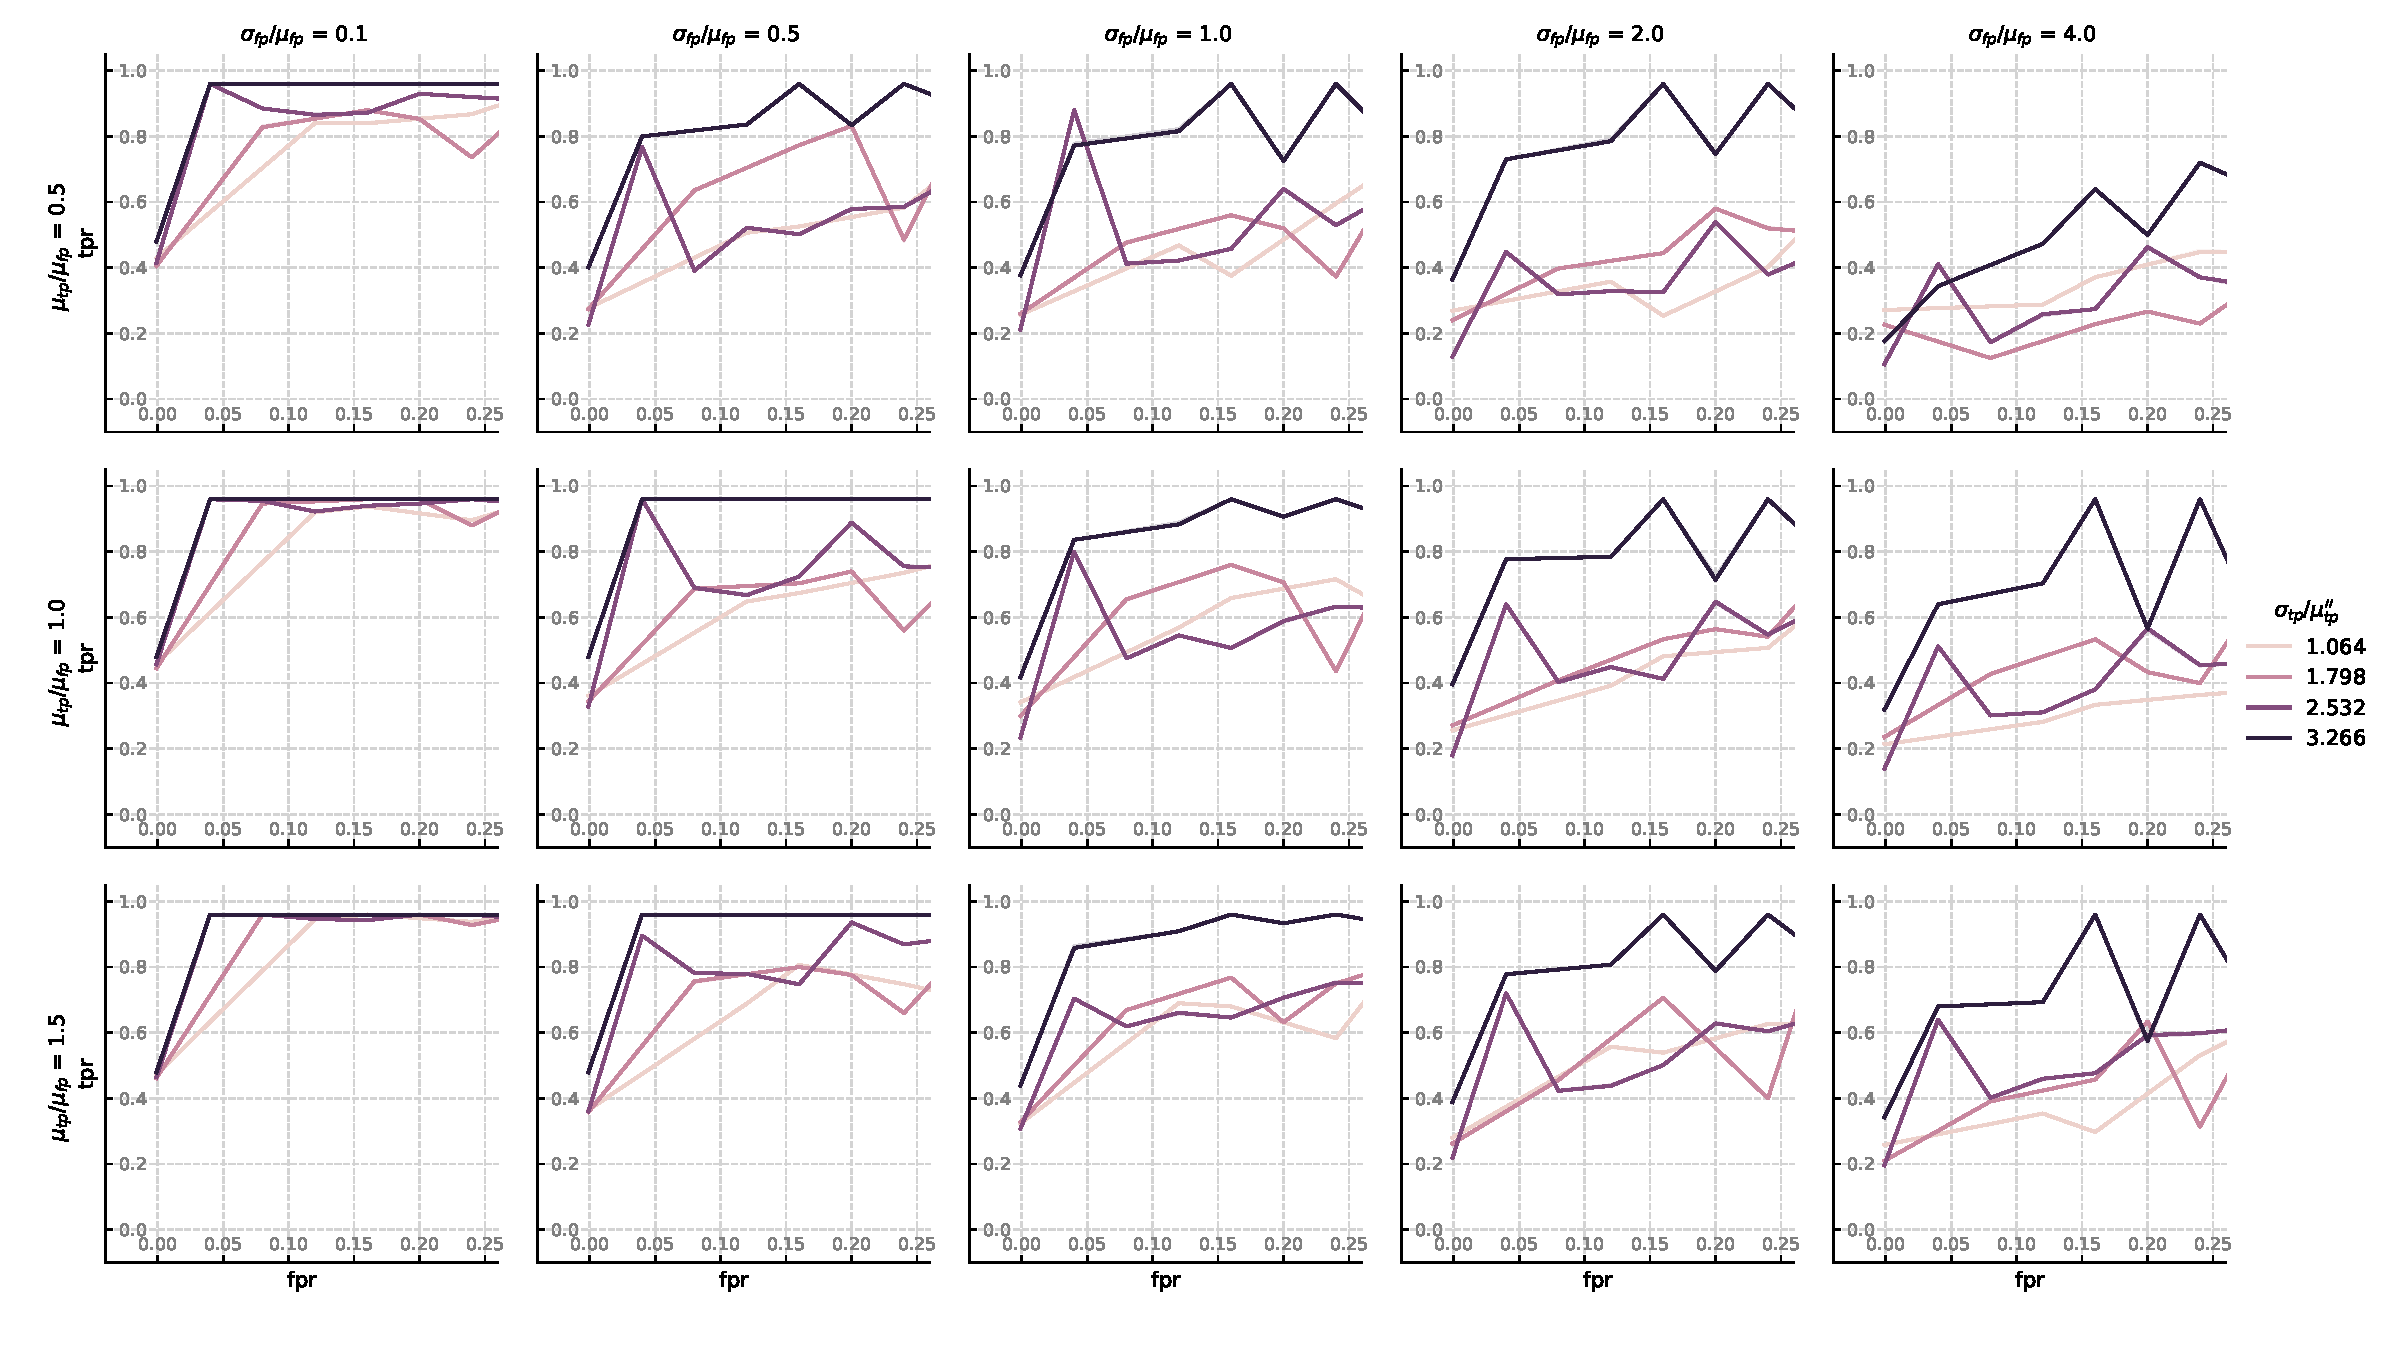
\includegraphics[width=\paperwidth]{simda.pdf}
        };
    \end{tikzpicture}
\end{frame}




\begin{frame}[plain]
    \begin{tikzpicture}[remember picture,overlay]
        \node[at=(current page.center)] {
            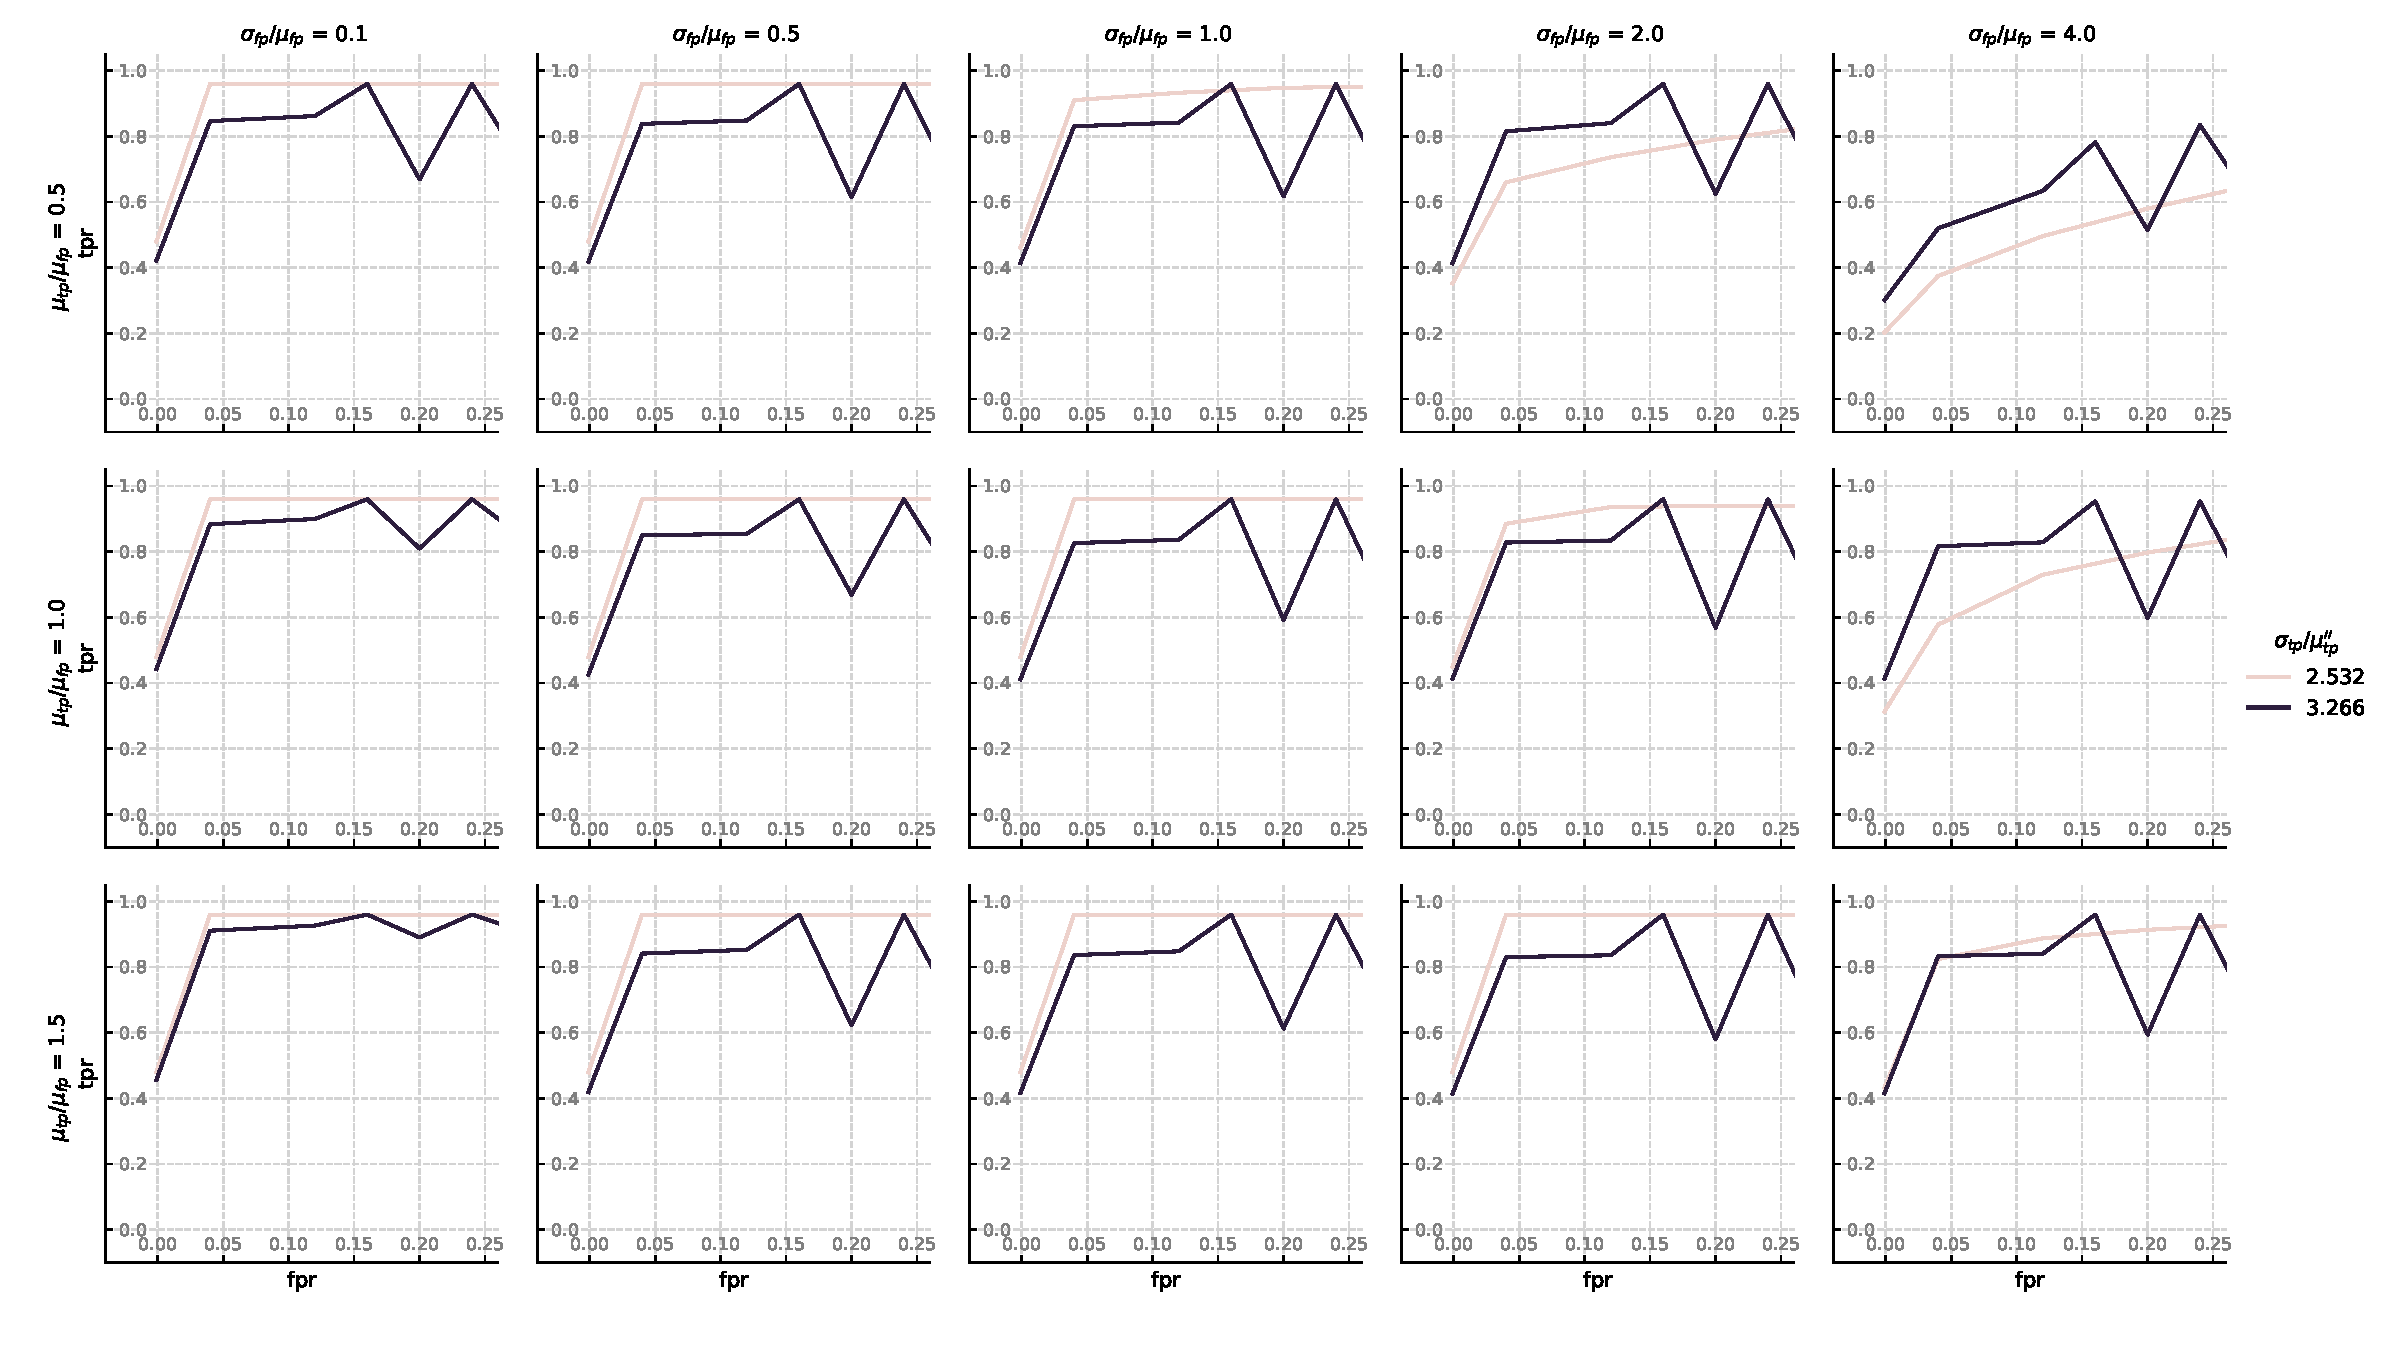
\includegraphics[width=\paperwidth]{unknown.pdf}
        };
    \end{tikzpicture}
\end{frame}



\begin{frame}[plain]
    \begin{tikzpicture}[remember picture,overlay]
        \node[at=(current page.center)] {
            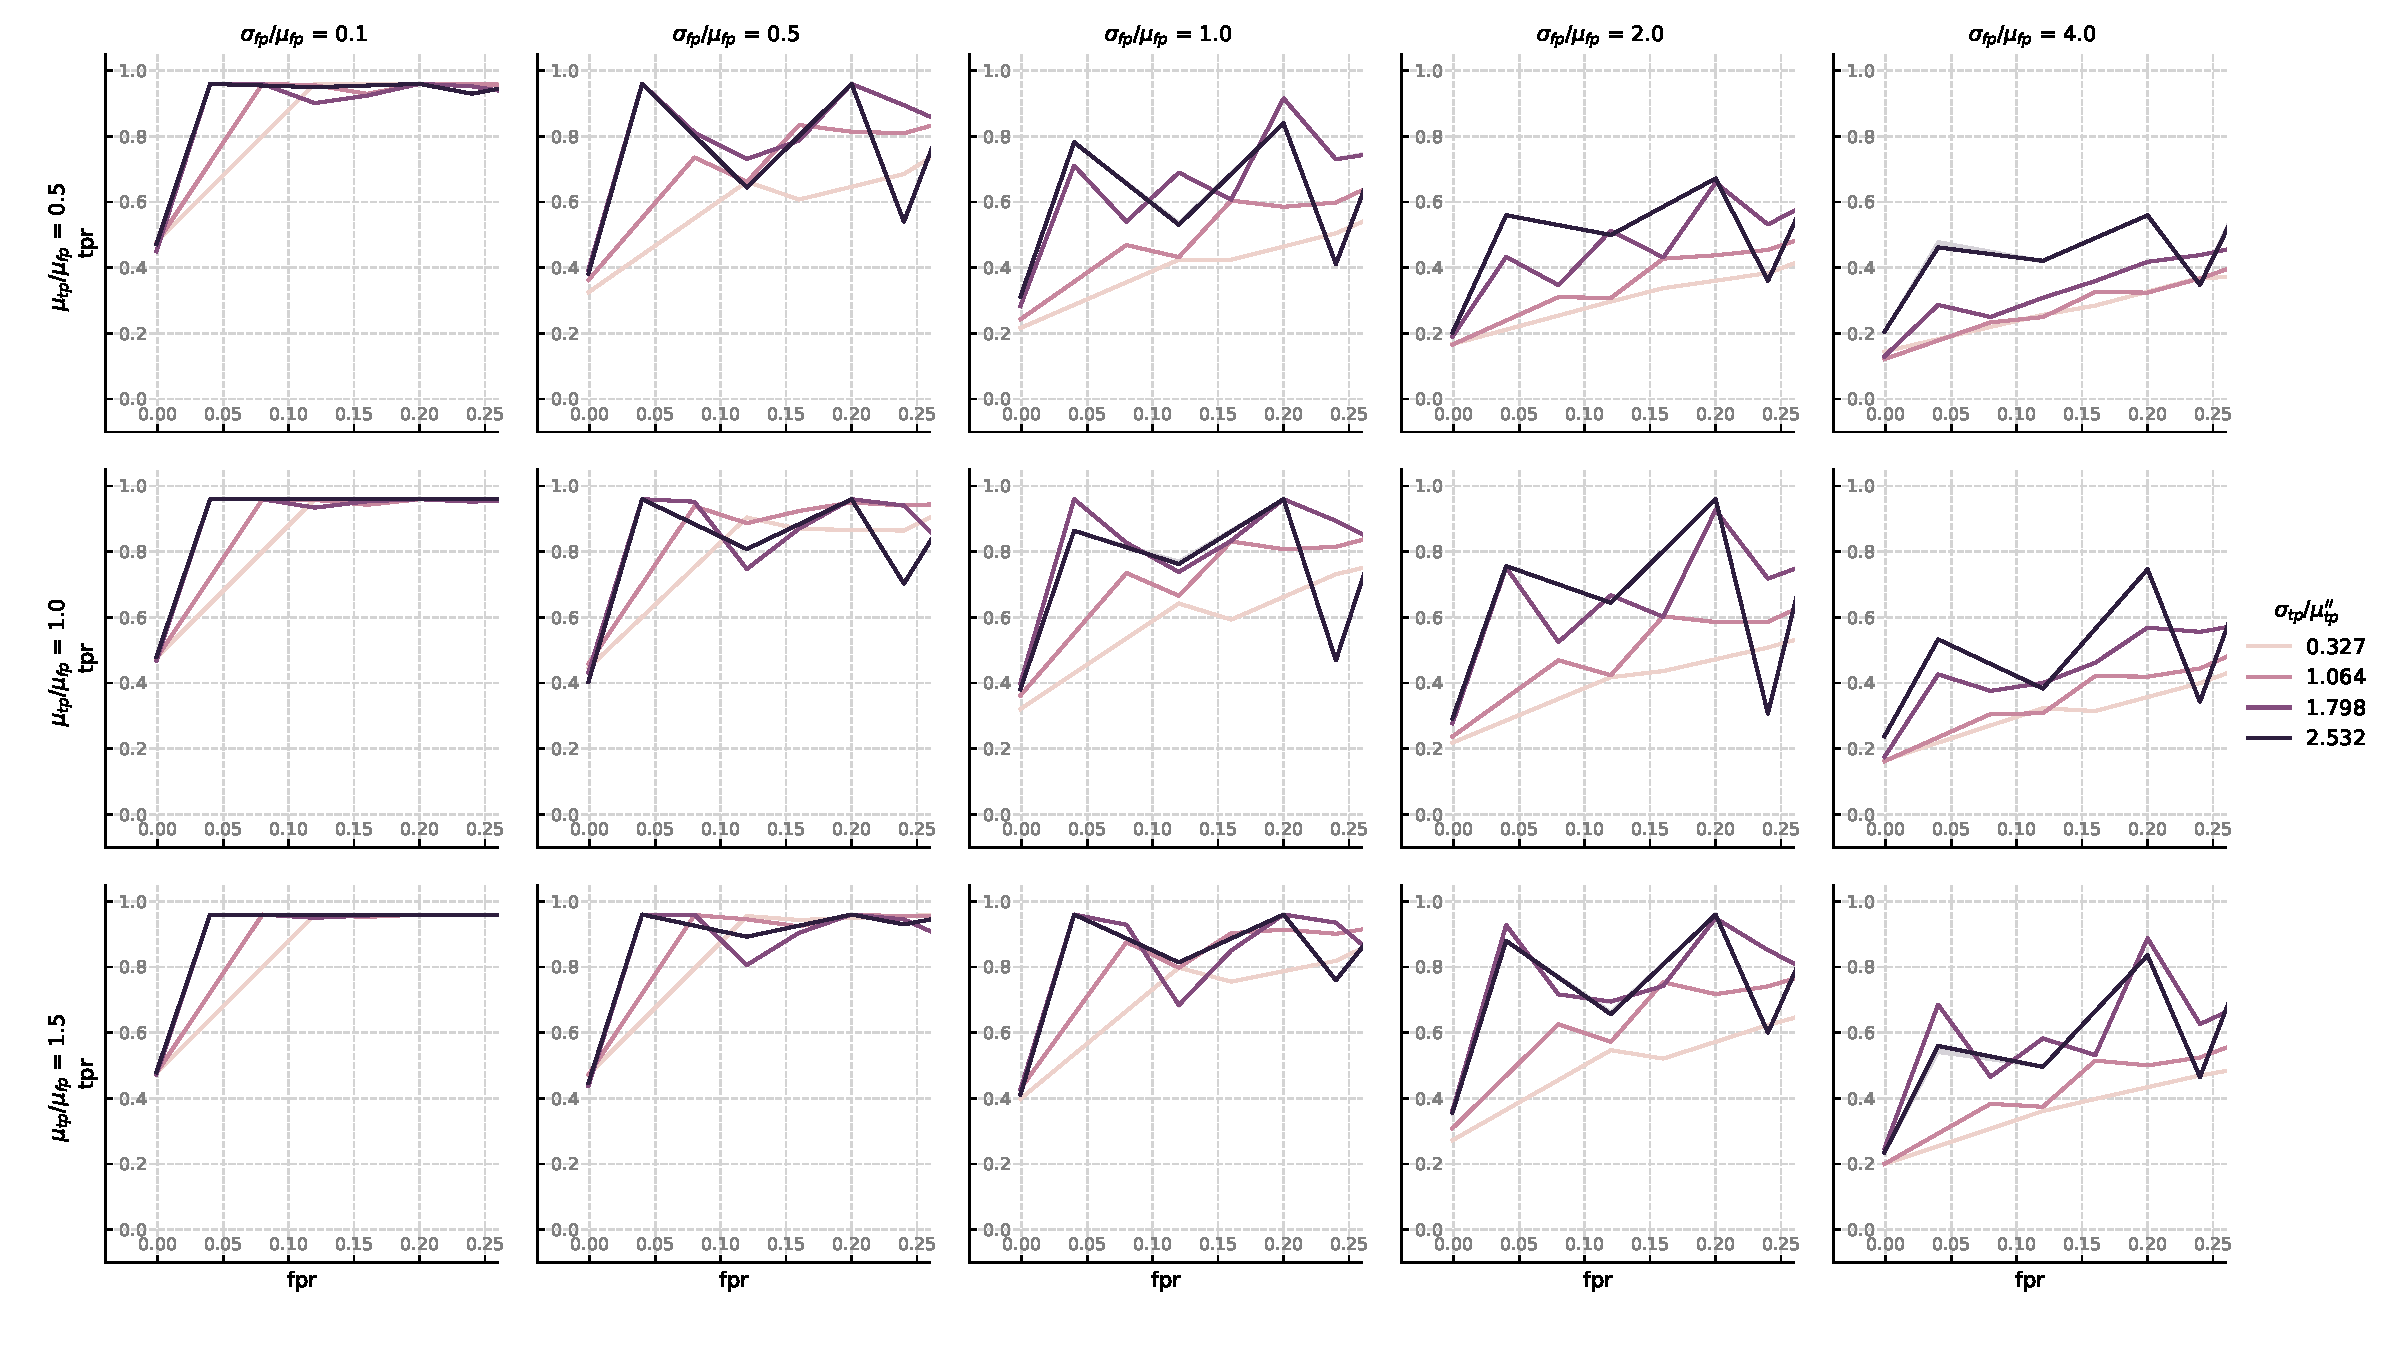
\includegraphics[width=\paperwidth]{zbot.pdf}
        };
    \end{tikzpicture}
\end{frame}


\end{document}
